\cotefile{156-5}
\scanpage{26}\mspage{25}
(resp. \unsure{ouvert|ouverte}, resp. loc. fer.) est idem.

Le cas d'une \deleted{\unsure{sur|su|sub}}subdivision est celui où $S=T$, i.e. s'explicite comme une situation
\diagram{\begin{tikzcd}[ampersand replacement=\&,row sep=large]
 S \arrow[r,hook] \arrow[d,"p"',"{\text{surj}}"] \& \mathcal L\\
 I \arrow[d,"\varphi"',"{\text{surj.}}"] \& {}\\
 J \& {,}
\end{tikzcd}}
% slanted; independent note at the left of the diagram
\margin{Attention au cas où $\varphi$ est bijective, sans être un iso (deux structures d'ordre diff. sur un $=$ $I$, avec l'une plus fine que l'autre). C'est le cas d'un $F\unsure{\preceq|\leq}G$, avec $F\ne G$, et pourtant $=$ relation \deleted{\unsure{d'éq}} $\unsure{\mathcal R|\mathscr R}_{F}=\mathcal R_{G}$ sur $|F|=|G|$.}
en posant $q=\varphi\unsure{\circ}p$.

\uline{Proposition} Soient $F,G$ deux figures.

% Unlabelled vertical marginal grouping stroke alongside a), forked at its lower end.
\margin{\figure{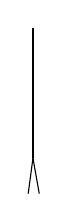
\begin{tikzpicture}[x=1cm,y=1cm]
\draw (0,0) -- (0,-1.65);
\draw (0,-1.65) -- (-0.06,-2.10);
\draw (0,-1.65) -- (0.08,-2.10);
\end{tikzpicture}}}
a) Pour que $F$ raffine $G$, il f et s que ce soit une sous-figure d'une \deleted{\unsure{raff|suf}}subdivision $G'$ de $F$
\[
 :\qquad F\leq G'\preceq G
\]

\deleted{b) Pour que $F$ soit une subdivision de $G$, il f et s. que ce soit un raffinement, et qu'il soit maximal comme}

\deleted{Ainsi, \unsure{dans|dès|donc} $F$}

\uline{Dém}. C'est \unsure{évid\(^{\mathrm{mt}}\)} suffisant, \unsure{Invers\(^{\mathrm{mt}}\)}, Supposons $F\ll G$, pour trouver $G'$, on prend $G'=G$ si $F$ est déjà une subd. i.e. $|F|=|G|$. \deleted{Sinon}, Dans le cas général, Soit
\[
\begin{aligned}
 G'&=\bigl\{A\in\unsure{\mathfrak P|\mathscr P|\mathbb P}(L)\mid A\in F\text{ ou }A=\deleted{\unsure{g}}\{x\},\text{ où }x\in |F|\unsure{\setminus}\,\unsure{G|F}\unsure{\}|,}\\
   &=F\coprod_{x\in |F|\setminus |G|}\{\{x\}\}
\end{aligned}
\]
